\begin{nolinenumbers}
\begin{table*}[htbp]
\centering
\caption{Main experimental results. Full results are in Appendix~\ref{app:main_results}. All values are average MAE and MAPE (\%) across all conditions. Red background: best result; blue background: second-best result.}
\label{tab:main_results}
\footnotesize
\setlength{\tabcolsep}{1.5pt}
\resizebox{\textwidth}{!}{%
\begin{tabular}{l | cc | cc | cc | cc | cc | cc | cc | cc | cc | cc | cc}
\toprule
& \multicolumn{2}{c|}{SE-TSA} & \multicolumn{2}{c|}{DLinear} & \multicolumn{2}{c|}{PatchTST} & \multicolumn{2}{c|}{TiDE} & \multicolumn{2}{c|}{TimeXer} & \multicolumn{2}{c|}{Kimi K2.6} & \multicolumn{2}{c|}{DeepSeek V4 Flash} & \multicolumn{2}{c|}{Gemma4 26B A4B} & \multicolumn{2}{c|}{Qwen3.6 35B A3B} & \multicolumn{2}{c|}{Moirai 2.0} & \multicolumn{2}{c}{TimeCopilot} \\
\cmidrule(lr){2-3} \cmidrule(lr){4-5} \cmidrule(lr){6-7} \cmidrule(lr){8-9} \cmidrule(lr){10-11} \cmidrule(lr){12-13} \cmidrule(lr){14-15} \cmidrule(lr){16-17} \cmidrule(lr){18-19} \cmidrule(lr){20-21} \cmidrule(lr){22-23}
Dataset & MAE & MAPE & MAE & MAPE & MAE & MAPE & MAE & MAPE & MAE & MAPE & MAE & MAPE & MAE & MAPE & MAE & MAPE & MAE & MAPE & MAE & MAPE & MAE & MAPE \\
\midrule
Agriculture & \best{5.97E+00} & \best{2.71} & 6.92E+00 & 3.12 & \second{6.06E+00} & \second{2.74} & 6.79E+00 & 3.04 & 6.60E+00 & 2.97 & 9.23E+00 & 4.18 & 8.24E+00 & 3.69 & 8.36E+00 & 3.72 & 7.31E+00 & 3.26 & 8.82E+00 & 3.98 & 9.20E+00 & 4.27 \\
Climate & \best{4.34E-01} & \best{17.88} & 4.98E-01 & 21.20 & \second{4.83E-01} & \second{19.95} & 5.06E-01 & 21.06 & 4.85E-01 & 20.08 & 5.40E-01 & 23.88 & 4.85E-01 & 20.75 & 4.97E-01 & 21.84 & 4.93E-01 & 21.21 & 5.50E-01 & 22.95 & 9.95E-01 & 40.77 \\
Economy & \best{8.27E+03} & \best{10.14} & 9.08E+03 & 11.56 & \second{8.67E+03} & \second{10.63} & 9.87E+03 & 12.26 & 9.21E+03 & 11.23 & 1.56E+04 & 18.44 & 1.61E+04 & 19.69 & 1.54E+04 & 18.15 & 1.48E+04 & 17.89 & 1.29E+04 & 15.82 & 1.09E+04 & 13.54 \\
Energy & \best{3.25E-01} & \best{10.07} & 4.06E-01 & 12.55 & 3.87E-01 & 11.95 & 3.80E-01 & 11.77 & 4.12E-01 & 12.74 & 5.04E-01 & 14.76 & 4.14E-01 & 12.16 & 4.13E-01 & 12.18 & 3.99E-01 & 11.94 & \second{3.49E-01} & \second{10.77} & 4.53E-01 & 14.43 \\
Environment & \best{2.10E+01} & \best{33.00} & 2.42E+01 & 37.29 & 2.39E+01 & 36.98 & 2.33E+01 & \second{33.96} & \second{2.30E+01} & 36.01 & NA & NA & NA & NA & NA & NA & NA & NA & 2.77E+01 & 41.91 & 2.93E+01 & 44.27 \\
PublicHealth & \best{9.80E-01} & \best{48.13} & 1.19E+00 & 64.64 & 1.54E+00 & 84.51 & 1.14E+00 & 56.20 & 1.53E+00 & 86.65 & 2.12E+00 & 118.30 & 1.25E+00 & 53.80 & 1.59E+00 & 73.73 & 1.36E+00 & 61.06 & \second{1.08E+00} & \second{48.90} & 1.85E+00 & 97.98 \\
Security & \best{1.63E+09} & 71.71 & 1.67E+09 & 73.75 & 1.78E+09 & 76.69 & 1.86E+09 & 80.81 & 1.70E+09 & 68.71 & 2.09E+09 & 78.06 & 1.81E+09 & 73.27 & 1.65E+09 & \best{66.54} & 1.74E+09 & \second{68.38} & \second{1.64E+09} & 73.06 & 1.71E+09 & 80.46 \\
SocialGood & \best{8.08E-01} & \best{12.83} & 8.30E-01 & 13.98 & 8.22E-01 & 13.61 & 8.57E-01 & 14.46 & \second{8.09E-01} & \second{13.44} & 1.28E+00 & 20.77 & 1.14E+00 & 17.92 & 1.23E+00 & 20.81 & 1.16E+00 & 17.44 & 8.78E-01 & 14.20 & 8.32E-01 & 13.59 \\
Traffic & \best{1.03E+04} & \best{4.31} & 1.66E+04 & 6.74 & \second{1.08E+04} & \second{4.49} & 1.61E+04 & 6.52 & 1.22E+04 & 5.03 & 2.60E+04 & 10.26 & 4.01E+04 & 15.62 & 2.92E+04 & 11.36 & 3.04E+04 & 11.95 & 2.38E+04 & 9.35 & 3.31E+04 & 12.99 \\
\bottomrule
\end{tabular}%
}
\end{table*}
\end{nolinenumbers}

\section{Experiments}

We adopt datasets compiled by Time-MMD~\cite{TimeMMD}, which include nine subsets from diverse domains, thereby enabling a comprehensive and fair comparison. Dataset descriptions and preprocessing details are provided in Appendix~\ref{app:implementation}. Forecasting performance is evaluated using two standard metrics, namely Mean Absolute Error (MAE) and Mean Absolute Percentage Error (MAPE):
\begin{equation}
\text{MAE} = \frac{1}{T} \sum_{t=1}^{T} \left\| \mathbf{\hat{X}}_{t+1:t+L_{\text{out}}}^{\text{endo}} - \mathbf{X}_{t+1:t+L_{\text{out}}}^{\text{endo}} \right\|,
\end{equation}
\begin{equation}
\text{MAPE} = \frac{100\%}{T} \sum_{t=1}^{T}
\frac
{\left\| \mathbf{\hat{X}}_{t+1:t+L_{\text{out}}}^{\text{endo}} - \mathbf{X}_{t+1:t+L_{\text{out}}}^{\text{endo}} \right\|}
{\left\| \mathbf{X}_{t+1:t+L_{\text{out}}}^{\text{endo}} \right\| },
\end{equation}
where $\mathbf{\hat{X}}_{t+1:t+L_{\text{out}}}^{\text{endo}}=\mathbf{\hat{X}}_{t+1:t+L_{\text{out}}}^{\text{ensemble}}$ and $\mathbf{X}_{t+1:t+L_{\text{out}}}^{\text{endo}}$ denote the predicted and ground-truth endogenous variables, respectively.

\subsection{Main Results}

Table~\ref{tab:main_results} summarizes the main experimental results across all benchmark datasets. The detailed result and benchmark settings can be found in Appendix~\ref{app:main_results}. SE-TSA and TimeCopilot use Kimi K2.6~\cite{Kimi} as LLM server.

Generally, SE-TSA achieves the best MAE performance on all nine datasets, demonstrating strong and consistent forecasting precision across diverse domains. For the MAPE metric, SE-TSA obtains the best results on eight datasets and underperforms Gemma4~\cite{Gemma} on the Security dataset ($71.71\%$ versus $66.54\%$).

It is worth noting that the absolute MAE values on some datasets are relatively large. This phenomenon primarily reflects the large numerical scale and strong non-stationarity of the original time series.

In contrast, direct LLM inference baselines consistently exhibit inferior performance. Moreover, smaller language models like Gemma4 26B A4B and Qwen3.6 35B A3B~\cite{Qwen} can outperform larger ones --- Kimi K2.6 and Deepseek V4~\cite{Deepseek} --- on certain datasets, suggesting that scaling model size alone does not effectively address time-series forecasting challenges.

Among the compared baselines, the time-series foundation model Moirai 2.0  and deep learning model PatchTST achieve competitive performance and attain the second-best results on several datasets. However, their performance remain inconsistent across different domains, whereas SE-TSA demonstrates substantially stronger robustness and generalization ability.

\begin{nolinenumbers}
\begin{table}[htbp]
\centering
\caption{Domain transfer results. Full results are in Appendix~\ref{app:domain_tranfer}. All values are average MAE and MAPE (\%) across all conditions. Red background: best result; blue background: second-best result.}
\label{tab:domain_transfer}
\small
\setlength{\tabcolsep}{2pt}
\resizebox{\columnwidth}{!}{%
\begin{tabular}{l | cc | cc | cc | cc | cc}
\toprule
\multicolumn{1}{r|}{Source} & \multicolumn{2}{c|}{Agriculture} & \multicolumn{2}{c|}{Climate} & \multicolumn{2}{c|}{Environment} & \multicolumn{2}{c|}{PublicHealth} & \multicolumn{2}{c}{Traffic} \\
\cmidrule(lr){2-3} \cmidrule(lr){4-5} \cmidrule(lr){6-7} \cmidrule(lr){8-9} \cmidrule(lr){10-11}
Target & MAE & MAPE & MAE & MAPE & MAE & MAPE & MAE & MAPE & MAE & MAPE \\
\midrule
Agriculture & \best{5.97E+00} & \best{2.71} & 1.19E+01 & 5.37 & 6.61E+00 & 2.97 & \second{6.00E+00} & \best{2.71} & 6.08E+00 & 2.75 \\
\midrule
Climate & 4.67E-01 & 19.37 & \best{4.34E-01} & \best{17.88} & \second{4.59E-01} & 19.12 & 4.66E-01 & 19.36 & 4.63E-01 & \second{19.04} \\
\midrule
Environment & 2.27E+01 & 34.92 & NA & NA & \best{2.10E+01} & \best{33.00} & \second{2.19E+01} & \best{33.00} & 2.24E+01 & 34.62 \\
\midrule
PublicHealth & \second{1.13E+00} & \second{54.74} & 7.86E+01 & 4363.87 & 1.18E+00 & 56.01 & \best{9.80E-01} & \best{48.13} & 1.20E+00 & 59.55 \\
\midrule
Traffic & \second{1.10E+04} & \second{4.59} & 1.48E+04 & 5.83 & 1.32E+04 & 5.48 & 1.14E+04 & 4.73 & \best{1.03E+04} & \best{4.31} \\
\bottomrule
\end{tabular}%
}
\end{table}
\end{nolinenumbers}

\subsection{Domain Transfer Analysis}

Table~\ref{tab:domain_transfer} presents the results of directly transferring the forecasting architectures obtained from one domain (dataset) to another domain.

Architectures evolved on a specific domain consistently achieve their best performance when evaluated on the same domain. For instance, the PublicHealth-evolved models achieve the best MAE of $0.980$ on PublicHealth, whereas transferring the Climate architectures to PublicHealth results in a dramatic degradation to $78.6$ MAE and $4363.87\%$ MAPE. Similarly, on the Traffic dataset, the in-domain architectures achieve an MAE of $1.03\times10^4$, outperforming transferred architectures by at least $6.4\%$.

These results indicate that the evolved architectures capture domain-specific characteristics. Therefore, SE-TSA does not merely identify generic forecasting structures, but instead automatically evolves architectures that are specialized for different datasets and domains.

\begin{nolinenumbers}
\begin{table}[htbp]
\centering
\caption{Ablation study results. Full results are in Appendix~\ref{app:ablation}. All values are average MAE and MAPE (\%) across all conditions. Red background: best result; blue background: second-best result.}
\label{tab:ablation}
\small
\setlength{\tabcolsep}{3pt}
\resizebox{\columnwidth}{!}{%
\begin{tabular}{l | cc | cc | cc | cc}
\toprule
& \multicolumn{2}{c|}{w/o Reflection} & \multicolumn{2}{c|}{w/o MAP-Elites} & \multicolumn{2}{c|}{w/o Ensemble} & \multicolumn{2}{c}{SE-TSA} \\
\cmidrule(lr){2-3} \cmidrule(lr){4-5} \cmidrule(lr){6-7} \cmidrule(lr){8-9}
Dataset & MAE & MAPE & MAE & MAPE & MAE & MAPE & MAE & MAPE \\
\midrule
Agriculture & \second{6.15E+00} & \second{2.76} & 6.67E+00 & 2.99 & 6.43E+00 & 2.90 & \best{5.97E+00} & \best{2.71} \\
Climate & \second{4.35E-01} & \second{18.00} & 4.52E-01 & 18.60 & 4.54E-01 & 18.60 & \best{4.34E-01} & \best{17.88} \\
Environment & \second{2.11E+01} & 33.13 & 2.12E+01 & \second{33.05} & 2.18E+01 & 34.45 & \best{2.10E+01} & \best{33.00} \\
PublicHealth & 1.06E+00 & 51.77 & \second{9.84E-01} & \best{47.81} & 9.91E-01 & 49.08 & \best{9.80E-01} & \second{48.13} \\
Traffic & 1.11E+04 & 4.63 & \second{1.05E+04} & 4.39 & \second{1.05E+04} & \second{4.37} & \best{1.03E+04} & \best{4.31} \\
\bottomrule
\end{tabular}%
}
\end{table}
\end{nolinenumbers}

\subsection{Ablation Study}

Table~\ref{tab:ablation} shows the result of ablation study by removing MAP-Elites (coupled with dual-strategy model generation), reflection, and ensemble.

In most cases, removing any module leads to increased MAE and MAPE, demonstrating the effectiveness of the complete agent system design. The extent of performance degradation differs across datasets, suggesting that different domains benefit from different modules of SE-TSA. For example, removing MAP-Elites (which also removes the difference between EXPLORE and EXPLOIT) causes the most significant percentage degradation of MAPE on Agriculture (MAPE from $2.71$ to $2.99$, with $10.3\%$ degradation). In contrast, removing MAP-Elites has little effect on PublicHealth, where the performance remains close to that of the full agent system. Despite these domain-specific differences, the complete SE-TSA consistently achieves the best or near-best performance across all datasets, demonstrating that the proposed modules can complement each other and jointly improve the effectiveness of SE-TSA.

\begin{nolinenumbers}
\begin{table}[htbp]
\centering
\caption{Representative design principles extracted during evolution.}
\label{tab:principles_by_domain}
\small
\setlength{\tabcolsep}{2pt}
\begin{tabular}{l>{\raggedright\arraybackslash}p{1.2cm}>{\raggedright\arraybackslash}p{4.5cm}}
\toprule
\textbf{Dataset} & \textbf{Attribute} & \textbf{Representative Principle} \\
\midrule
Climate & Short seq, small & Shallow ODE networks outperform deeper configurations on climate forecasting; continuous-time modeling benefits from simple dynamics functions rather than expressive ODE solvers. \\
\midrule
Security & Short seq, small, irregular & Small linear models outperform attention-based and hybrid architectures by 10--100$\times$. \\
\midrule
Environment & Long seq, 41 features, periodic & Multi-scale wavelet decomposition outperforms neural basis expansion. \\
\midrule
PublicHealth & Medium seq, 44 features, periodic & Real-valued FFT projections enable effective attention mechanisms on small datasets. \\
\midrule
Traffic & Short seq, 17 features, small & Cross-channel attention mechanisms catastrophically fail on small traffic datasets, performing 6$\times$ worse than channel-independent models. \\
\bottomrule
\end{tabular}
\end{table}
\end{nolinenumbers}

\subsection{Case Study}

Table~\ref{tab:principles_by_domain} lists the most representative principle from each dataset, selected to highlight how the evolved knowledge directly reflects the data's intrinsic properties. More case analysis can be found in Appendix~\ref{app:case_study}.

\subsubsection{Dataset Characteristics and Design Principles}

The principles reveal a direct correspondence between data characteristics and architectural choices. Small dataset (Climate) favor compact continuous-time models, whereas long-horizon, high-dimensional data (Environment) require multi-scale wavelet decomposition. Small-sample irregular data (Security) tend to converge toward simple linear models, while periodic multi-feature data (PublicHealth) benefit from real-valued frequency-domain preprocessing to facilitate attention mechanisms. Besides, small-sample traffic data (Traffic) exhibit catastrophic degradation under cross-channel interaction modeling. These observations suggest that the reflection mechanism adapts to the underlying data structure.

\subsubsection{Cross-Domain Principle Contrast}

We observe that similar design principles can lead to opposite outcomes depending on domain characteristics. For instance, feature interaction modeling fails dramatically on small low-dimensional datasets such as Traffic, yet becomes effective on high-dimensional datasets like PublicHealth when combined with appropriate preprocessing.

Moreover, simple linear models outperform attention-based architectures on small irregular datasets such as Security, whereas deep multi-scale decomposition is crucial for long-horizon high-dimensional datasets like Environment. These findings suggest that the appropriate level of model complexity should align with the underlying data distribution and structural properties of the dataset.

\begin{nolinenumbers}
\begin{figure}[htbp]
  \centering
  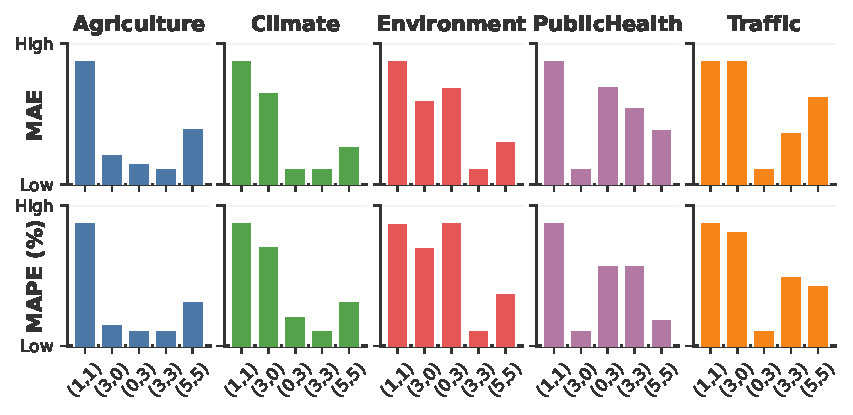
\includegraphics[width=\columnwidth]{figures/Hyperparam.pdf}
  \caption{Hyperparameter analysis of ensemble. Full results are in Appendix~\ref{app:hyperparam}.}
  \label{fig:hyperparam}
\end{figure}
\end{nolinenumbers}

\subsection{Hyperparameter Analysis of Ensemble Configuration}

The forecasting performance of SE-TSA is influenced by the ensemble module. To analyze its sensitivity, we evaluate five different $(N_{1}, N_{2})$ configurations: $(1,1)$, $(3,0)$, $(0,3)$, $(3,3)$, and $(5,5)$, where $(3,3)$ is the default setting.

As shown in Figure~\ref{fig:hyperparam}, the default $(3,3)$ achieves the superior performance on most datasets. In contrast, the single-source configurations ($(3,0)$ and $(0,3)$) yield inferior results. These observations indicate the effectiveness of jointly leveraging globally optimal models and behaviorally diverse elites. Although $(5,5)$ further increases the ensemble size, its performance does not improve consistently, likely because the additional models are relatively low-quality candidates.